\chapter{Regression}
\section{Evaluating Regression Models Performance}
R square
\begin{equation}
SS_{hot}=SUM(y_i-y_{avg})^2
\end{equation}
\begin{equation}
SS_{hot}=SUM(y_i-y_{avg})^2
\end{equation}
\begin{equation}
R^2=1-\frac{SS_{res}}{SS_{tot}}
\end{equation}
Here, we want $SS_{res} \rightarrow Min$

The problem here is: if we have $n$ features (regressor) have been already existed in our regression model. We will add a new feature, we want to know if it helps to improve the performance of hour model. The solution is: we compare the difference of $R^2$ with and without the new feature. There are two situations here:
\begin{enumerate}
	\item $R^2$ increase. Because the new feature decrease the $SS_{res}$
	\item $R^2$ keeps unchanged. Because the new feature does not help the model. It has no effect on the dependant variable. The coefficient of the new feature is zero.
\end{enumerate}
When add a new feature, it is bias as the $R^2$ is always increase. So the adjust $R$ square is proposed.
\begin{equation}
Adj R^2 = 1- (1 - R^2)\frac{n-1}{n-p-1},
\end{equation}
where $p$ is the number of regressors and $n$ is the sample size.

One example is shown as follows:
\begin{figure}
	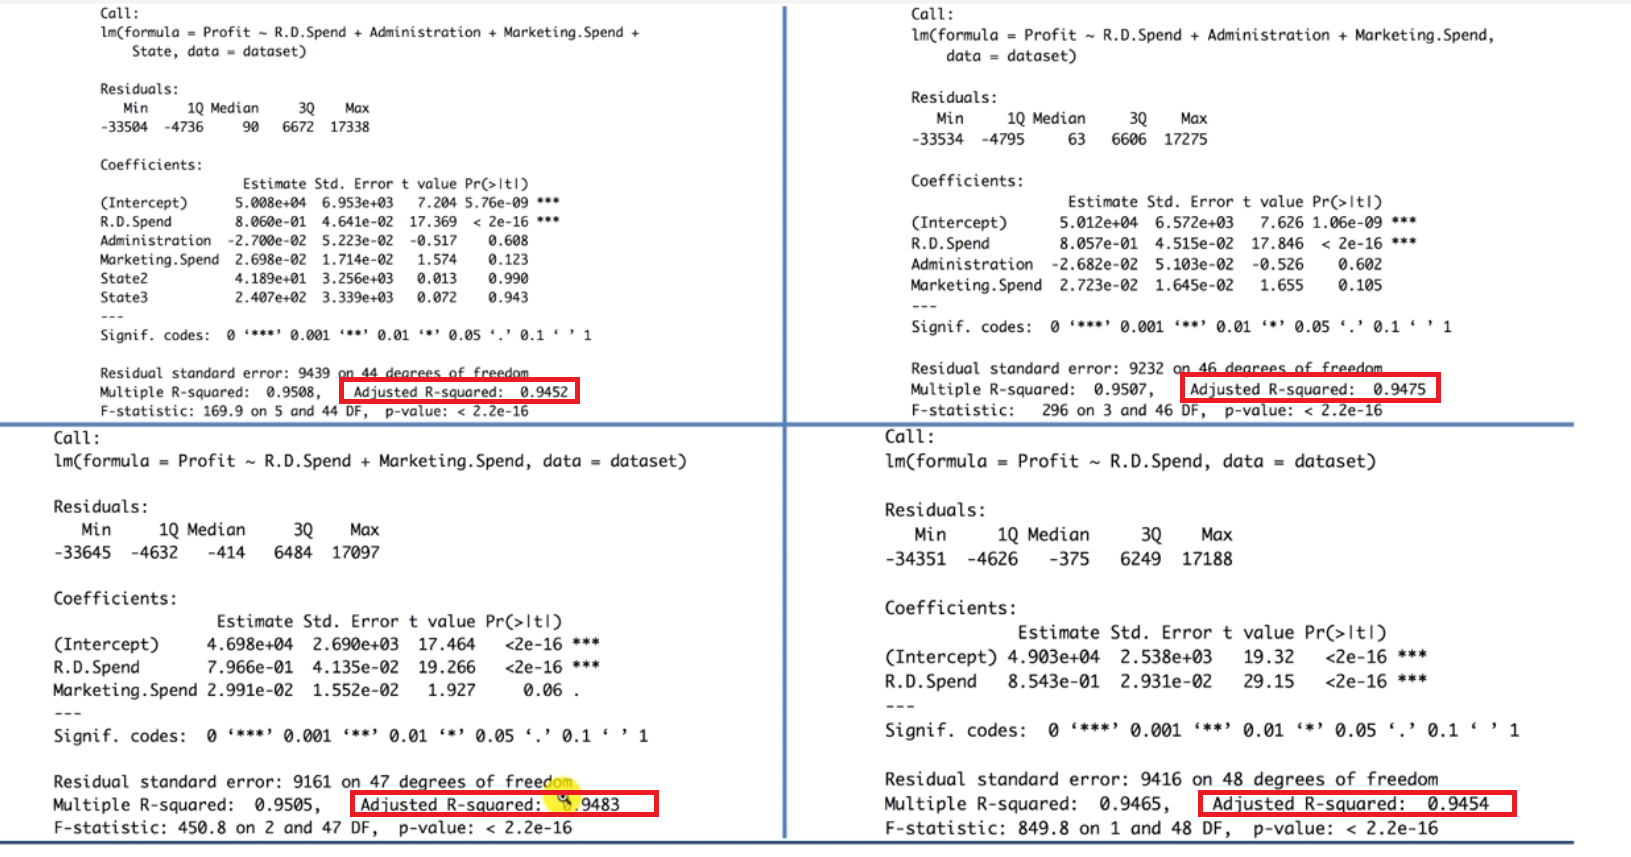
\includegraphics[width=\linewidth]{./figures/adjust_r_square.png}
	\centering
	\caption{example of adjust square error}
\end{figure}

\begin{table}
	\begin{tabular}{ | C{0.33\linewidth} | C{0.33\linewidth}| C{0.33\linewidth} | } 
		\hline
		Regression Model & Pros & Cons \\ 
		\hline
		Linear Regression &  Works on any size of dataset, gives information about relevance of features & The Linear Regression Assumptions \\
		\hline 
		Polynomial Regression & works on any size of dataset, works very well on non linear problems & Need to choose the right polynomial degree for a good bias/variance tradeoff \\ 
		\hline
		SVR & Easily adaptable, works very well on non linear problems, not biased by outliers & Compulsory to apply feature scaling, not well known, more difficult to understand \\
		\hline
		Decision Tree Regression & Interpretability, no need for feature scaling, works on both  linear/nonlinear problems & Poor results on too small datasets, overfitting can easily occur\\
		\hline
		Random Forest Regression & powerful and accurate, good performance on many problems, including non linear & Nointerpretability, overfitting can easily occur, need to choose the number of trees\\
		\hline
	\end{tabular}
\caption{Comparison of different regression models}
\label{table:comp}
\end{table}
Table \ref{table:comp} shows the comparison of different regression models from  \href{https://www.superdatascience.com/wp-content/uploads/2017/02/Regression-Pros-Cons.pdf}{comparison}.

How to address overfitting problems:\href{https://www.superdatascience.com/wp-content/uploads/2017/02/Regularization.pdf}{Regularization}.
